% Copyright (c) 2012 Raniere Silva <r.gaia.cs@gmail.com>
% Copyright (c) 2012 Fernando Cezarino <feolce@gmail.com>
% Copyright (c) 2012 Ana Paula Diniz Marques <anapdinizm@gmail.com>
% Copyright (c) 2012 Camile Kunz <camileknz@gmail.com>
% Copyright (c) 2012 Ana Flavia <anaflavia.c.lima@gmail.com>
%
% This file is part of 'MS480 - 2012S2 - Aterro com Obstáculo'.
%
% 'MS480 - 2012S2 - Aterro com Obstáculo' is licensed under the Creative
% Commons Attribution-ShareAlike 3.0 Unported License. To view a copy of
% this license, visit http://creativecommons.org/licenses/by-sa/3.0/.
%
% 'MS480 - 2012S2 - Aterro com Obstáculo' is distributed in the hope
% that it will be useful, but WITHOUT ANY WARRANTY; without even the
% implied warranty of MERCHANTABILITY or FITNESS FOR A PARTICULAR
% PURPOSE.

\section{Modelagem}
A seguir apresentamos a modelagem proposta por Andjel e depois expandimos essa
modelagem para o problema a ser tratado. Ao final, abordamos a questão da
distância.

\subsection{Problema sem obstáculo}
Considere a Figura~\ref{fig:ilust_J_A} em que é ilustrado as regiões $J$ e
$A$.
\begin{figure}[!htb]
    \centering
    \begin{tikzpicture}
        \draw[pattern=bricks] (0,0) -- (0,3) -- (2,2) -- (4,0) -- (0,0);
        \node[fill=white] at (1,1) {$A$};
        \draw[pattern=checkerboard] (6,6) -- (8,6) -- (8,8) -- (6,8) -- (5,7) --
        (6,6);
        \node[fill=white] at (7,7) {$J$};

        % Escala
        \node[fill=white, above] at (5,1.2) {$0$};
        \draw[fill=black] (5,1) rectangle (6,1.2) node[fill=white, above]{$e$};
        \draw[fill=white] (6,1) rectangle (7,1.2) node[fill=white, above]{$2e$};
        \draw[fill=black] (7,1) rectangle (8,1.2) node[fill=white, above]{$3e$};
    \end{tikzpicture}
    \caption{Ilustra\c{c}\~{a}o das regiões $J$ e $A$.}
    \label{fig:ilust_J_A}
\end{figure}

Para modelarmos o problema, discretizamos a região ilustrada na
Figura~\ref{fig:ilust_J_A} utilizando uma malha quadriculada como, ilustrado na
Figura~\ref{fig:disc_J_A}, e nomeamos cada quadrado da malha por um número
seguindo a lógica parcialmente indicada na Figura~\ref{fig:disc_J_A}.
\begin{figure}[!htb]
    \centering
    \begin{tikzpicture}
        \draw[color=gray, step=.5] (0,0) grid (8,8);
        \draw[pattern=bricks] (0,0) -- (0,3) -- (2,2) -- (4,0) -- (0,0);
        \node[fill=white] at (1,1) {$A$};
        \draw[pattern=checkerboard] (6,6) -- (8,6) -- (8,8) -- (6,8) -- (5,7) --
        (6,6);
        \node[fill=white] at (7,7) {$J$};

        \draw[pattern=bricks](0,0) rectangle (2,2) node[fill=white,
        midway]{$A$};
        \draw[pattern=checkerboard] (6,6) rectangle (8,8) node[fill=white,
        midway]{$J$};

        \foreach \x in {1,...,11}{
            \node at (\x/2 - .25,7.75) {\small{$\x$}};
        }
        \foreach \x in {17,...,26}{
            \node at (\x/2 - 8.25,7.25) {\small{$\x$}};
        }

        % Escala
        \node[fill=white, above] at (5,1.2) {$0$};
        \draw[fill=black] (5,1) rectangle (6,1.2) node[fill=white, above]{$e$};
        \draw[fill=white] (6,1) rectangle (7,1.2) node[fill=white, above]{$2e$};
        \draw[fill=black] (7,1) rectangle (8,1.2) node[fill=white, above]{$3e$};
    \end{tikzpicture}
    \caption{Ilustra\c{c}\~{a}o das regiões $J$ e $A$.}
    \label{fig:disc_J_A}
\end{figure}

Pela Figura~\ref{fig:disc_J_A} \'{e} poss\'{i}vel observar que alguns elementos
da malha quadriculada encontram-se apenas parcialmente dentro de uma das
regi\~{o}es. Para corrigir isso, aproximamos as regi\~{o}es para a malha
utilizada de modo que todos os elementos da malha que encontram-se parcialmente
presentes em uma das regi\~{o}es passa a pertencer totalmente a ela. O resultado
\'{e} apresentado na Figura~\ref{fig:disc_J_A_aprox}.
\begin{figure}[!htb]
    \centering
    \begin{tikzpicture}
        \draw[color=gray, step=.5] (0,0) grid (8,8);
        \draw[pattern=bricks] (0,0) -- (0,3) -- ++(1,0) -- ++(0,-.5) -- ++(1,0)
        -- ++(0,-.5) -- ++(.5,0) -- ++(0,-.5) -- ++(.5,0) -- ++(0,-.5) --
        ++(.5,0) -- ++(0,-.5) -- ++(.5,0) -- ++(0,-.5) -- (4,0) -- (0,0);
        \node[fill=white] at (1,1) {$A$};
        \draw[pattern=checkerboard] (6,6) -- (8,6) -- (8,8) -- (6,8) --
        ++(-.5,0) -- ++(0,-.5) -- ++(-.5,0) -- ++ (0,-.5) -- ++(0,-.5) --
        ++(.5,0) -- ++(0,-.5) -- ++(.5,0) -- (6,6);
        \node[fill=white] at (7,7) {$J$};

        \draw[pattern=bricks](0,0) rectangle (2,2) node[fill=white,
        midway]{$A$};
        \draw[pattern=checkerboard] (6,6) rectangle (8,8) node[fill=white,
        midway]{$J$};

        % Escala
        \node[fill=white, above] at (5,1.2) {$0$};
        \draw[fill=black] (5,1) rectangle (6,1.2) node[fill=white, above]{$e$};
        \draw[fill=white] (6,1) rectangle (7,1.2) node[fill=white, above]{$2e$};
        \draw[fill=black] (7,1) rectangle (8,1.2) node[fill=white, above]{$3e$};
    \end{tikzpicture}
    \caption{Ilustra\c{c}\~{a}o das regiões $J$ e $A$.}
    \label{fig:disc_J_A_aprox}
\end{figure}

Seja $\phi : J \to \mathbb{R}$, $\psi: A \to \mathbb{R}$, $f: (J, A) \to
\mathbb{R}$ e $d: (J, A) \to \mathbb{R}$, onde $\phi(x)$ corresponde ao volume
de terra disponível no quadrado $x$, $\psi(y)$ ao volume de terra necessário no
quadrado $y$, $f(x, y)$ ao volume de terra transportado do quadrado $x$ para o
quadrado $y$ e $d(x, y)$ a distância entre os quadrados $x$ e $y$.

Sendo $\xi_{x, y} = f(x, y)$ a variável de decisão, podemos modelar o problema
da seguinte forma:
\begin{subequations}
    \begin{align}
        \text{max } & \sum_{x} \sum_{y} \xi_{x, y},
        \label{eq:model_without_obs:obj_func} \\
        \text{s.a. } & \xi_{x, y} \geq 0, && \forall x, y,
        \label{eq:model_without_obs:var} \\
        & \xi_{x, y} = 0, && \forall (x, y) | d(x, y) > D,
        \label{eq:model_without_obs:max_dist} \\
        & \sum_{y} \xi_{x, y} \leq \phi(x), && \forall x,
        \label{eq:model_without_obs:max_jazida} \\
        & \sum_{x} \xi_{x, y} \leq \psi(y), && \forall y,
        \label{eq:model_without_obs:max_aterro}
    \end{align}
    \label{eq:model_without_obs}
\end{subequations}
onde $x \in J$, $y \in A$, \eqref{eq:model_without_obs:max_dist} refere-se a
distância máxima dos canos utilizados, \eqref{eq:model_without_obs:max_jazida} a
quantidade de terra que pode ser retirado de $J$ e
\eqref{eq:model_without_obs:max_aterro} a quantidade de terra necessário em $A$.

O modelo apresentado em \eqref{eq:model_without_obs} possue função objetivo e
restrições lineares. Em relação a restrição
\eqref{eq:model_without_obs:max_dist}, como $d(x, y)$ é um dado do problema
o conjunto $\left\{ (x, y) | d(x, y) > D \right\}$ é gerado dinamicamente ao
construir os dados para uma dada instância do problema.

\subsection{Problema com obstáculo}
Considerando que a região $R$ pela qual os canos que fazem o transporte da terra
não podem passar é circular, com centro $c = (c_1, c_2) \in \mathbb{R}^2$ e raio
$r \in \mathbb{R}$. Então temos a região de interesse ilustrada na
Figura~\ref{fig:disc_J_A_R}.
\begin{figure}[!htb]
    \centering
    \begin{tikzpicture}
        \draw[color=gray, step=.5] (0,0) grid (8,8);
        \draw[->] (-.2,8) -- (8.2,8);
        \draw[->] (0,-.2) -- (0,8.2);

        \draw[color=gray, step=.5] (0,0) grid (8,8);
        \draw[pattern=bricks] (0,0) -- (0,3) -- ++(1,0) -- ++(0,-.5) -- ++(1,0)
        -- ++(0,-.5) -- ++(.5,0) -- ++(0,-.5) -- ++(.5,0) -- ++(0,-.5) --
        ++(.5,0) -- ++(0,-.5) -- ++(.5,0) -- ++(0,-.5) -- (4,0) -- (0,0);
        \node[fill=white] at (1,1) {$A$};
        \draw[pattern=checkerboard] (6,6) -- (8,6) -- (8,8) -- (6,8) --
        ++(-.5,0) -- ++(0,-.5) -- ++(-.5,0) -- ++ (0,-.5) -- ++(0,-.5) --
        ++(.5,0) -- ++(0,-.5) -- ++(.5,0) -- (6,6);
        \node[fill=white] at (7,7) {$J$};
        \draw[pattern=fivepointed stars] (4,4) node[fill=white]{$R$}
        circle (1.7) ;

        % Escala
        \node[fill=white, above] at (5,1.2) {$0$};
        \draw[fill=black] (5,1) rectangle (6,1.2) node[fill=white, above]{$e$};
        \draw[fill=white] (6,1) rectangle (7,1.2) node[fill=white, above]{$2e$};
        \draw[fill=black] (7,1) rectangle (8,1.2) node[fill=white, above]{$3e$};
    \end{tikzpicture}
    \caption{Ilustra\c{c}\~{a}o da malha quadricular sobre a regi\~{a}o de
    interesse.}
    \label{fig:disc_J_A_R}
\end{figure}

Seja $P$ a região que não corresponde a jazida, ao aterro e nem ao obstáculo.
De maneira semelhante as definições utilizadas na subseção anterior, seja $\phi
: J \to \mathbb{R}$, $\psi: A \to \mathbb{R}$, $f: (J, P, A) \to \mathbb{R}$,
$d: (J \cup A, P) \to \mathbb{R}$ e $l: (J \cup A, P) \to \mathbb{R}$, onde
$\phi(x)$ corresponde ao volume de terra disponível no quadrado $x$, $\psi(y)$
ao volume de terra necessário no quadrado $y$, $f(x, z, y)$ ao volume de terra
transportado do quadrado $x$ para o quadrado $y$ passando pelo quadrado $z$,
$d(w, z)$ a distância entre os quadrados $w$ e $z$\footnote{A distância entre os
quadrados $w$ e $z$ será definida posteriormente.} e $l(w, z)$ a distância entre
a reta formada pelos quadrados $w$ e $z$ ao ponto $c$\footnote{A distância entre a
reta formada pelos quadrados $w$ e $z$ ao ponto $c$ é abordada no
Apêndice~\ref{sse:point2line}.}.

Sendo $\xi_{x, z, y} = f(x, z, y)$ a variável de decisão, podemos modelar o
problema da seguinte forma:
\begin{subequations}
    \begin{align}
        \text{max } & \sum_{x} \sum_{z} \sum_{y} \xi_{x, z, y},
        \label{eq:model_with_obs_nl:obj_func} \\
        \text{s.a. } & \xi_{x, z, y} \geq 0, && \forall x, z, y,
        \label{eq:model_with_obs_nl:var} \\
        & \xi_{x, z, y} = 0, && \forall (x, z, y) | d(x, z) > D \text{ ou } 
        d(y, z) > D,
        \label{eq:model_with_obs_nl:max_dist} \\
        & \xi_{x, z, y} = 0, && \forall (x, z, y) | l(x, z) < r \text{ ou }
        l(y, z) < r,
        \label{eq:model_with_obs_nl:dist_obs} \\
        & \sum_{y} \xi_{x, z, y} \leq \phi(x), && \forall x, z,
        \label{eq:model_with_obs_nl:max_jazida} \\
        & \sum_{x} \xi_{x, z, y} \leq \psi(y), && \forall z, y,
        \label{eq:model_with_obs_nl:max_aterro}
    \end{align}
    \label{eq:model_with_obs_nl}
\end{subequations}
onde $x \in J$, $y \in A$, $z \in P$, \eqref{eq:model_with_obs_nl:max_dist}
refere-se a distância máxima dos canos utilizados,
\eqref{eq:model_with_obs_nl:dist_obs} a restrição dos canos não passar pela
região $R$, \eqref{eq:model_with_obs_nl:max_jazida} a quantidade de terra que pode
ser retirado de $J$ e \eqref{eq:model_with_obs_nl:max_aterro} a quantidade de terra
necessário em $A$.

O modelo apresentado em \eqref{eq:model_with_obs_nl} possue função objetivo e
restrições lineares. Em relação as restrições
\eqref{eq:model_with_obs_nl:max_dist} e \eqref{eq:model_with_obs_nl:dist_obs},
como $d(x, z)$, $d(y, z)$, $l(x, z)$ e $l(y, z)$ são dados do problema os
conjuntos $\left\{ (x, z, y) | d(x, z) > D \text{ ou } d(y, z) > D \right\}$ e
$\left\{ (x, z, y) | l(x, z) < r \text{ ou } l(y, z) < r \right\}$ são gerados
dinamicamente ao construir os dados para uma dada instância do problema.

Seria interessante poder lidar com regiões $R$ mais gerais. Uma forma de fazer
isso é aproximar a região $R$ utilizando o mesmo procedimento adotado para
aproximar as regiões $J$ e $A$. O resultado da aproximação da região $R$ é
ilustrada na Figura~\ref{fig:disc_J_A_R_aprox}.
\begin{figure}[!htb]
    \centering
    \begin{tikzpicture}
        \draw[color=gray, step=.5] (0,0) grid (8,8);
        \draw[->] (-.2,8) -- (8.2,8);
        \draw[->] (0,-.2) -- (0,8.2);

        \draw[color=gray, step=.5] (0,0) grid (8,8);
        \draw[pattern=bricks] (0,0) -- (0,3) -- ++(1,0) -- ++(0,-.5) -- ++(1,0)
        -- ++(0,-.5) -- ++(.5,0) -- ++(0,-.5) -- ++(.5,0) -- ++(0,-.5) --
        ++(.5,0) -- ++(0,-.5) -- ++(.5,0) -- ++(0,-.5) -- (4,0) -- (0,0);
        \node[fill=white] at (1,1) {$A$};
        \draw[pattern=checkerboard] (6,6) -- (8,6) -- (8,8) -- (6,8) --
        ++(-.5,0) -- ++(0,-.5) -- ++(-.5,0) -- ++ (0,-.5) -- ++(0,-.5) --
        ++(.5,0) -- ++(0,-.5) -- ++(.5,0) -- (6,6);
        \node[fill=white] at (7,7) {$J$};
        \draw[pattern=fivepointed stars] (3,2.5) -- ++(0,-.5) -- ++(2,0) --
        ++(0,.5) -- ++ (.5,0) -- ++(0,.5) -- ++(.5,0) -- ++(0,2) -- ++ (-.5,0)
        -- ++(0,.5) -- ++(-.5,0) -- ++(0,.5) -- ++(-2,0) -- ++(0,-.5) --
        ++(-.5,0) -- ++(0,-.5) -- ++(-.5,0) -- ++(0,-2) -- ++(.5,0) -- ++(0,-.5)
        -- (3,2.5);
        \node[fill=white] at (4,4) {$R$};

        % Escala
        \node[fill=white, above] at (5,1.2) {$0$};
        \draw[fill=black] (5,1) rectangle (6,1.2) node[fill=white, above]{$e$};
        \draw[fill=white] (6,1) rectangle (7,1.2) node[fill=white, above]{$2e$};
        \draw[fill=black] (7,1) rectangle (8,1.2) node[fill=white, above]{$3e$};
    \end{tikzpicture}
    \caption{Ilustra\c{c}\~{a}o da malha quadricular sobre a regi\~{a}o de
    interesse.}
    \label{fig:disc_J_A_R_aprox}
\end{figure}

O modelo a ser utilizado ao utilizar a aproximação da região $R$ é semelhante a
\eqref{eq:model_with_obs_nl} mudando apenas a restrição
\eqref{eq:model_with_obs_nl:dist_obs} que passa a ser
\begin{align}
    % \xi_{x, z, y} &= 0, && \forall (x, z, y) | b(x, z) \notin R \text{ ou }
    % b(y, z) \notin R,
    \xi_{x, z, y} &= 0, && \forall (x, z, y) | b(x, z) \neq 1 \text{ ou }
    b(y, z) \neq 1,
    \label{eq:model_with_obs:dist_obs} 
\end{align}
onde $b: (J \cup A, P) \to \left\{ 0, 1 \right\}$ é $1$ se a linha reta
construída entre os quadrados $w \in J \cup A$ e $z \in P$ utilizando o
algoritmo de Bresenham\footnote{Ver o Apêndice~\ref{sse:bresenham_line}.} passa
por $R$ e $0$ caso contrário.

\subsection{Distância entre pontos}
Ao utilizar a malha quadriculada podemos definir a dist\^{a}ncia entre dois
quadrados da malha de pelo menos tr\^{e}s maneiras diferentes:
\begin{enumerate}
    \item $d_l$, que \'{e} a menor dist\^{a}ncia entre qualquer dois pontos dos
        quadrados,
    \item $d_u$, que \'{e} a maior dist\^{a}ncia entre qualquer dois pontos dos
        quadrados, e
    \item $d_c$, que \'{e} a dist\^{a}ncia entre os centros dos quadrados.
\end{enumerate}
Na Figura~\ref{fig:dist_malha} \'{e} ilustrado cada uma das dist\^{a}ncias acima
descrita.
\begin{figure}[!htb]
    \centering
    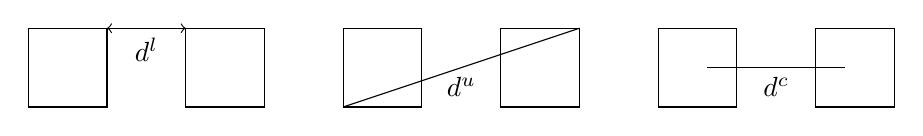
\begin{tikzpicture}
        \draw (0,0) rectangle (1,1);
        \draw (2,0) rectangle (3,1);
        \draw[<->] (1,1) -- (2,1) node[midway, below]{$d^l$};

        \draw (4,0) rectangle (5,1);
        \draw (6,0) rectangle (7,1);
        \draw (4,0) -- (7,1) node[midway, below]{$d^u$};

        \draw (8,0) rectangle (9,1) node[midway](A){};
        \draw (10,0) rectangle (11,1) node[midway](B){};
        \draw (A) -- (B) node[midway, below]{$d^c$};
    \end{tikzpicture}
    \caption{Ilustra\c{c}\~{a}o das dist\^{a}ncias entre quadrados da malha.}
    \label{fig:dist_malha}
\end{figure}
